\RequirePackage[T1]{fontenc}
\documentclass[conference,10pt,letterpaper]{IEEEtran}
\usepackage{amsmath,amssymb,graphicx,booktabs,cite}
\usepackage{algorithm,algpseudocode,tikz}
\usetikzlibrary{arrows.meta,positioning}
\usepackage[hidelinks]{hyperref}
\hypersetup{pdfauthor={},pdftitle={Exposing Inter-Sample and Intra-Search Parallelism in Layer-Aware Lookahead Construction for 3D FPGA Routing}}
\makeatletter
\newcommand{\tableinput}[1]{\@@input #1 }
\makeatother
\newtheorem{proposition}{Proposition}
\newcommand{\LstmPipeBuild}{$3.207\pm0.147\times$}
\newcommand{\LstmPipeProc}{$1.094\pm0.010\times$}
\newcommand{\LstmFlatBuild}{$3.208\pm0.165\times$}
\newcommand{\LstmFlatProc}{$1.092\pm0.007\times$}
\newcommand{\LstmAltCpuBuild}{$3.167\pm0.071\times$}
\newcommand{\LstmAltCpuProc}{$1.088\pm0.000122\times$}
\newcommand{\LstmStockBuild}{$21.182\pm1.342\times$}
\newcommand{\LstmStockProc}{$1.839\pm0.049\times$}
\newcommand{\StageProcBound}{1.005435}

\title{Exposing Inter-Sample and Intra-Search Parallelism in Layer-Aware Lookahead Construction for 3D FPGA Routing}
\author{\IEEEauthorblockN{Anonymous Authors}}
\begin{document}\maketitle
\begin{abstract}
Layer-aware lookahead construction can dominate multicore FPGA routing workflows. We expose two levels of parallelism through separate execution contracts: STRICT schedules independent samples with private workspaces and ordered reduction, while ALT uses whole-pair FP32 bucket waves within each search. The native integration preserves layer and source identity while explicitly separating semantic guarantees. Existing eight-core GEMM measurements show 1.638-fold process acceleration for STRICT Pipeline. On a preselected same-family LSTM case, ALT CUDA accelerates native construction by 3.207-fold and the complete process by 1.094-fold against Pipeline. We report congestion differences, checked routing quality, and small-input slowdowns; FPGA hardware superiority remains unverified.
\end{abstract}
\begin{IEEEkeywords}3D FPGA, routing lookahead, parallel CAD, CPU/GPU, execution contracts\end{IEEEkeywords}
\section{Introduction}
Three-dimensional FPGA architecture exploration depends on CAD tools that represent layer-dependent connectivity and evaluate it at practical cost. LaZagna enables flexible 3D architecture generation, and Escaping Flatland improves placement for stacked fabrics~\cite{lazagna,flatland}. These developments motivate faster routing initialization: evaluating a changed resource graph or calibrated cost model can require reconstructing the heuristic used by timing-driven routing. A multicore router alone does not remove sequential work from this construction.

In our locked VPR baseline, the map-lookahead builder floods representative wire starts sequentially. On eight-core GEMM, construction accounts for approximately 45\% of the complete fixed-input process: its mean time is 149.56 seconds, compared with 30.64 seconds for routing. Parallelizing independent starts is attractive because the graph and indexed cost model remain read-only. However, a group often has only four samples. A barrier between groups limits useful concurrency even when sixteen physical cores are available. Parallelism within a single search offers another opportunity, but changes the order in which tied delay/congestion labels are selected.

We distinguish these opportunities through two explicit contracts. STRICT preserves the native within-flood visitation and original-order sample reduction while scheduling searches across groups. ALT introduces a separate FP32 whole-pair bucket/wave search, implemented on CPU and CUDA, beneath the same native sample interface. ALT does not inherit STRICT's equivalence proposition. We evaluate its semantic differences and downstream routing quality separately instead of conflating CPU/GPU agreement with native equivalence.

The contributions are: (1) a layer-aware STRICT decomposition into independent samples, private state and ordered reduction, with a scoped wire-map equivalence argument; (2) an independent ALT search contract exposing intra-search parallelism through snapshot waves and whole-pair updates; and (3) native system validation connecting construction to complete Process time, including a same-family tuning holdout, qualified routes and size-dependent negative results. Bucket algorithms, atomic operations and task libraries are established mechanisms; our contribution is their scoped integration and validation for this lookahead problem.

The principal GPU result is relative to optimized CPU Pipeline, rather than Stock: on LSTM, ALT CUDA achieves \LstmPipeBuild\ native construction acceleration and \LstmPipeProc\ Process acceleration. This is a CPU/GPU CAD implementation for FPGA targets. FPGA hardware acceleration is not a measured result.

\section{Problem and Related Work}
\subsection{Layer-Aware Samples and Native Costs}
A routing-resource graph $G=(V,E)$ represents wires, pins and switches. PathFinder-style negotiation resolves net contention~\cite{pathfinder}; VPR's timing-driven router combines accumulated costs with lookahead estimates~\cite{vtr8,vtr9}. Sampled wire maps retain representative costs by displacement~\cite{diversity}. For layered fabrics, a map cell is
\begin{equation}
F[\ell_s,\ell_t,c,s,\Delta x,\Delta y]=(d,q),
\end{equation}
where source/target layers, channel type and segment type identify the slice, and $(d,q)$ is the associated delay/congestion pair. Each group $g=(\ell_s,s,c)$ contains an ordered list of sample starts. One sample may reach destinations on every layer. Unoccupied cells are completed by native interpolation; source/OPIN preprocessing and derived minima are additional construction work.

Our graphs model two active layers with logic, DSP and memory resources, plus explicit vertical wires and inter-layer switches. They adopt the existing VTR 3D/multi-die modeling approach~\cite{third_dimension,multidie}. The qualified LSTM CUDA route uses 23,217 distinct CHANZ nodes. Thus the evaluated 3D scope includes actual vertical connectivity and routed paths, not just layer annotations. We retain the existing indexed cost model; this work does not introduce physical delay calibration or placement-delay refinement.

\subsection{Parallelism and Prior Algorithms}
Let $t_{g,j}$ be the ideal search work of sample $j$ in group $g$, $W_g=\sum_j t_{g,j}$, and $W=\sum_g W_g$. With $P$ workers, ideal group-local and global search times obey
\begin{align}
T_{\rm group}&\geq\sum_g\max\{W_g/P,\max_j t_{g,j}\},\\
T_{\rm global}&\geq\max\{W/P,\max_{g,j}t_{g,j}\}.
\end{align}
For ten groups of four equal-cost samples, eight workers need ten group-local waves but five global waves. Sixteen workers still need ten group-local waves, versus three global waves. This is a task-width example, not a utilization measurement or an optimal-scheduling guarantee. Memory bandwidth, reset, allocation and reduction add costs omitted from these bounds.

MultiQueue routing parallelizes individual connection searches through relaxed priority ordering~\cite{multiqueue}; STRICT instead leaves each flood's visitation unchanged. ALT shares the objective of exposing search parallelism but operates during heuristic construction rather than negotiated connection routing. We do not transfer serial-equivalence results from connection-search algorithms to ALT's delay/congestion map semantics.

Parallel bucket scheduling is established. Delta-stepping groups tentative distances to trade ordering against parallelism~\cite{delta}; GPU SSSP methods also balance work saving, frontier expansion and reorganization~\cite{gpu_sssp}. Our implementation differs in its native layer/source recording interface, whole delay/congestion pair selection, FP32 bit-key scheduling, same-bucket closure and target-cell completion. It is not a claim to invent bucketing or GPU SSSP, and it does not establish a new general SSSP complexity bound. oneTBB Pipeline and global parallel loops are similarly existing execution mechanisms~\cite{tbb}; the STRICT contribution is the dependency boundary that permits their use without changing the native wire table.

\section{Two Execution Contracts}
\subsection{A Common Native Task Boundary}
The native builder enumerates the original samples and supplies source RR identity, source-relative cell mapping, target-layer identity, CSR connectivity and indexed costs. Each backend returns sample cost pairs to the outer builder. The host retains group commit, interpolation and source/OPIN/minimum work. Both paths use this interface, but their search order and within-sample representative selection differ. This distinction prevents a shared interface from being mistaken for shared semantics.

Source identity is essential. Consider starts at $x=0$ and $x=5$ reaching a pin at $x=6$ with delays 1 and 2. They populate displacement buckets 6 and 1. A multi-source search retaining only the cheaper pin label loses the second contribution. We therefore preserve separate logical samples, including their coordinate contexts. Allocation reuse is allowed; reusing a previous sample's mutable labels or cached answer is not.

\begin{figure}[t]\centering
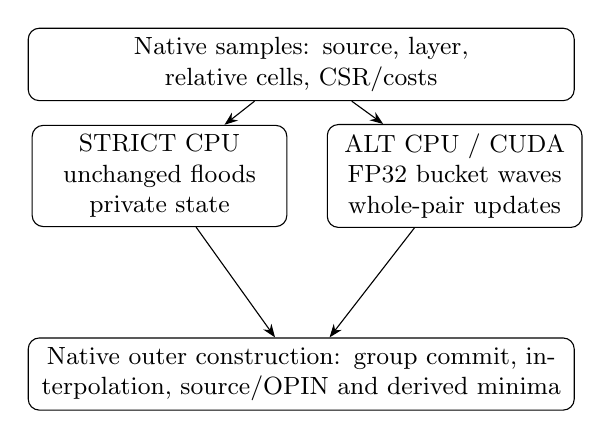
\begin{tikzpicture}[node distance=3mm, every node/.style={draw,rounded corners,align=center,font=\small,text width=6.7cm},>=Stealth]
\node (a) {Native samples: source, layer, relative cells, CSR/costs};
\node[below=of a,text width=3cm,xshift=-1.8cm] (b) {STRICT CPU\\unchanged floods\\private state};
\node[right=5mm of b,text width=3cm] (c) {ALT CPU / CUDA\\FP32 bucket waves\\whole-pair updates};
\node[below=16mm of a,yshift=-14mm] (d) {Native outer construction: group commit, interpolation, source/OPIN and derived minima};
\draw[->] (a)--(b);\draw[->] (a)--(c);\draw[->] (b)--(d);\draw[->] (c)--(d);
\end{tikzpicture}
\caption{Shared sample boundary with separate search contracts. STRICT's equivalence conditions do not extend to ALT. Diagram is conceptual.}\label{fig:contracts}\end{figure}

\subsection{STRICT: Private Floods, Ordered Reduction}
Each worker owns a visited-cost array, expanded bitmap, priority queue and sample output. Read-only graph/cost data are shared. The workspace is reset before every sample. Groups preserve X/Y/Z channel filtering and all destination-layer slices. Sample search uses the native full-device bounding box and existing edge/cost operations.

The native smallest-entry rule replaces a populated cell only for a strictly smaller delay. Congestion belongs to the winning delay; it must not be minimized independently. For finite occupied representatives, the winning sample is the earliest minimum-delay sample in native enumeration order:
\begin{equation}
j^*(u)=\arg\min_{j\,\mathrm{occupied}}(d_{g,j}(u),j).
\end{equation}
Implementation uses the native insertion and occupancy predicates, including missing-state behavior, rather than generic tuple sorting.

\begin{proposition}
If native sample selection and within-flood visitation are unchanged, valid recorded delays are finite, and final commits/interpolation follow native order, private sample execution followed by original-order strict-delay reduction yields the native wire-cost table.
\end{proposition}
\noindent\emph{Proof.} Each private flood produces the same per-cell representative as its native flood. Serial execution concatenates the visitation sequences in sample order. Original-order reduction selects the minimum delay and retains the earliest associated congestion on ties. Occupancy agrees cell by cell; identical commits and interpolation preserve that agreement. Task completion order does not enter the argument. $\square$

The proposition does not permit arbitrary exceptional-value reassociation, changed heap tie order or altered recording contexts. It also concerns the wire map, not every derived source/OPIN object or eventual routing trajectory. These boundaries matter when comparing independently repaired executables.

Group executes samples concurrently but waits at each group boundary. Pipeline exposes all groups through a bounded stream with parallel search and original-order reduction; reusable private workspaces avoid repeated allocation. Flat is an independent globally flattened parallel-loop control, not VPR's separate flat-routing option. Distinct layer/type/segment slices permit disjoint work, but interpolation within a slice follows its native dependency/order. Compact storage and alternative commit schedules are secondary variants, not assumed prerequisites of the reported native GPU result.

\subsection{ALT: Whole-Pair FP32 Bucket Waves}
ALT\_BUCKET\_FP32\_V1 is a separate contract. Admitted costs and accumulated candidates must be positive normal FP32 values or positive zero (negative zero and subnormals are rejected); unsupported numerics or capacity failures return an error without publishing a partial map. The unchanged native admission includes $N<2^{23}$. Labels begin at $(+\infty,+\infty)$ except source $(0,0)$; missing output cells retain their designated missing state.

For labels $a,b$, strict improvement means
\begin{equation}
a\prec b\iff a_d<b_d\ \lor\ (a_d=b_d\land a_q<b_q).
\end{equation}
The entire pair is selected. For nonnegative finite floats, CUDA packs the delay bits above congestion bits in a 64-bit word, allowing an unsigned atomic minimum to select one actual pair. It never combines a delay from one path with congestion from another. FP32 additions use round-to-nearest with contraction disabled in the matched implementations.

Scheduling uses $B(d)=\mathrm{bits}_{32}(d)\gg s$. We fix $s=20$ for the native experiments. Shift coarsens scheduling buckets, not stored delays: labels and returned costs remain FP32. At shift zero, the schedule key is the exact nonnegative FP32 delay bit key; this fact alone does not make ALT equivalent to native tie semantics.

A wave selects the smallest pending bucket, filters stale notifications and takes the current labels as its snapshot. All eligible outgoing edges generate proposals from that snapshot. Per-destination proposals begin from the existing label and reduce whole pairs; labels are committed only after expansion completes. Strictly improved destinations are published to their new bucket, including reinsertion into the current bucket. Pending deduplication avoids losing same-bucket notifications; old notifications are filtered on extraction. Closure occurs only when no pending work remains in the selected bucket. Target cells are recorded after closure, using whole-pair selection, and completion is tested then.

\begin{algorithm}[t]\caption{ALT wave contract (one logical sample)}\label{alg:alt}
\begin{algorithmic}[1]
\State Reset labels, pending state and outputs; publish source
\While{pending work exists and target cells incomplete}
\State Select minimum pending bucket $b$; filter stale members
\State Read wave-start labels; generate eligible proposals
\State Reduce each destination by whole-pair $\prec$
\State Commit strict improvements; publish or deduplicate
\If{bucket $b$ has no remaining work}
\State Record closed target cells; test target completion
\EndIf
\EndWhile
\State Return complete output or explicit failure
\end{algorithmic}\end{algorithm}

The original CPU implementation uses a sparse bucket directory and per-wave proposal storage. Basic CUDA uses dense pending-directory scans, parallel frontier expansion, atomic proposal selection and launch barriers between expansion, commit and closure. It is a matched native implementation, not a claim of optimal GPU SSSP. Reset, scans, synchronization and output handoff have real costs. Finite iteration/work/capacity guards prevent an unbounded run; an aborted invocation is not a successful timing sample. Exhaustion or target completion after closure terminates a successful search. We assert neither native tie equivalence nor universal routing-quality preservation for this contract.

\section{Experimental Method and Evidence}
\subsection{Frozen Inputs, Cohorts and Resources}
We reuse completed experiments; paper integration adds no solver or performance runs. The STRICT corpus has 603 formal records, comprising 414 legal full-flow and 189 construction-only observations. Construction-only studies use capped route tails and do not establish legal routes. The old CPU representative GEMM cohort and core-scaling cohort remain separate. Existing failed large-input route qualifications are retained in their attempted denominators rather than replaced by successful seeds.

The native ALT study has two further cohorts. R6.1 measures BNN and s38417 with Stock, Flat, ALT CPU and original live ALT CUDA. R6.2 preselects LSTM seed2 before ALT shift/cache/selector tuning and measures Stock, Flat, Pipeline, ALT CPU and original ALT CUDA on one new worker. R6.2 contains 43 managed runs: 33 formal timings, nine qualifications and one non-formal profile, not 43 extra formal performance repetitions. Its old-case Pipeline supplements and later CUDA conversion pairs belong to separate phases and are never paired post hoc.

LSTM is a tuning holdout within a previously studied family: it already appears in the CPU project's qualified width120 subset. It shares the architecture SHA with BNN, but has different netlist, placement, RRG and actual CSR/cost/job/cell/target inputs. LSTM has 4,166,724 nodes, 40,142,314 edges and 40 samples; BNN has 4,102,608 nodes, 39,480,616 edges and 40 samples. Both use two layers and width120. These are not independent-architecture generalization tests.

The locked CPU baseline is VTR commit \texttt{0b912334fdd8}, with release builds and assertion level 2. CPU experiments use Xeon Gold 6530 instances, physical-core affinity within one NUMA node, and the stated per-cohort worker budget. Native ALT runs use one H100 80GB GPU and eight distinct physical CPU cores, with sequential solver execution. Instances are shared; exclusivity is not established. R6.2 rotates arm order across three independent processes on each frozen input. Host, command, environment, binary/library hashes and input identities are bound in the artifact; different hosts and phases are not pooled.

\subsection{Timing and Statistical Policy}
E1 is the sample solver service interval; the reused CUDA wrapper ends its E1/service field before the final ABI output copy. E2 is the full native \texttt{MapLookahead::compute}: conversion, backend preparation/service, ordered group merge, interpolation, source/OPIN and derived-minimum work. E2 includes the output handoff. Process additionally includes RR XML loading, initialization, routing, checking/STA and uniform map serialization. Independent route readback is outside Process. Pre-generated RRG, packing and placement are excluded; filesystem caches are not flushed, so no cold-disk claim is made.

For paired repeat $r$, $s_r=T_{c,r}/T_{a,r}$. We report $\bar s=\sum_rs_r/n$ and sample SD $[\sum_r(s_r-\bar s)^2/(n-1)]^{1/2}$. Raw seconds also use mean and sample SD. Ratios are calculated before averaging; no products of unrelated speedups are reported. The three processes are runtime repeats, not three designs or placement seeds. SD is observed variability, not a confidence interval. Stock E2 uses its native log's 0.01-second print precision; other E2 values use the high-resolution constructor timer. Diagnostic capture, complete CPU/CUDA pair verification and the directed profile are excluded from formal timing.

\subsection{Semantic and Routing Qualification}
STRICT checks compare native wire-map bytes under the proposition's scope. ALT qualification separately checks complete same-input CPU/CUDA sample pairs and final map identity, then candidate-specific routing. Each route retains its own SHA through an independent original-VPR FULL/STA check, has zero overuse, and meets CPD and wirelength within $+5\%$ of the paired control. LSTM is checked against both Flat and Stock. This is measured qualification on frozen inputs, not an arbitrary-input QoR theorem.

A read-only audit explains the diagnosed isolated outer-boundary CHANZ subset from exact coordinate-generation rules and final in/out degrees. No graph is silently repaired and no errors are filtered. This explains that diagnostic subset, not all RRG invariants. The two CPU bounding-box notification repairs are object-bound in the reused integration. Stock and repaired C1 can have identical wire maps but different routing iterations: map identity excludes changes to that object, not all derived SOURCE/OPIN state or route history. Existing diagnostics do not establish a unique complete root cause. Thus Stock speedups describe the implementation combination; shared-repair Flat/Pipeline/ALT comparisons better isolate the construction change.

\section{Results and System Interpretation}
\subsection{STRICT Cross-Sample Parallelism}
On eight-core GEMM, STRICT Pipeline reduces mean construction from 149.56 to 20.95 seconds and obtains $1.638\pm0.005\times$ paired Process speedup versus Stock. Group reaches 37.88 seconds but remains limited by group barriers. This example motivates exposing independent tasks before changing a search algorithm. It does not imply that every VPR routing mode or circuit has the same bottleneck.

\begin{figure*}[t]\centering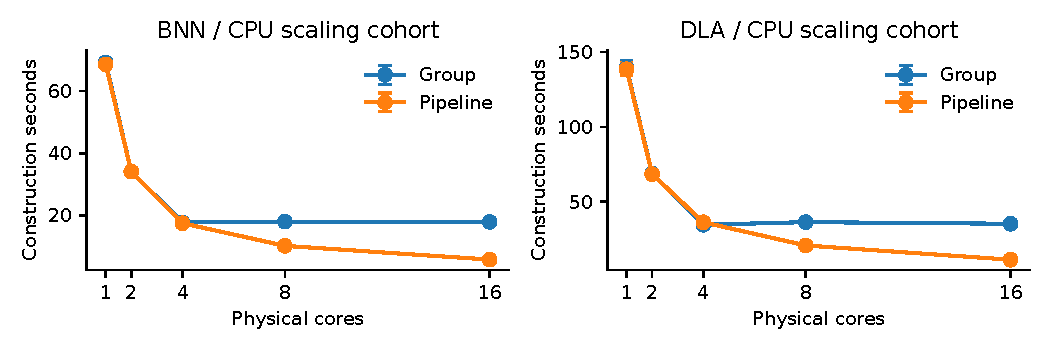
\includegraphics[width=.96\textwidth]{figures/scaling.pdf}
\caption{STRICT CPU construction-only core scaling, separate host-B cohort. Means and sample SD from three fixed-input processes per point. Group retains per-group barriers; Pipeline exposes global samples. Capped-routing tails do not establish legal full routes.}\label{fig:scale}\end{figure*}

Figure~\ref{fig:scale} illustrates why task width matters. On BNN and DLA, ten nonempty groups provide four samples each. Pipeline continues benefiting beyond four cores while Group saturates. A separate Flat global-loop control in the CPU evidence shows that removing group barriers, rather than the oneTBB Pipeline primitive alone, supplies the main concurrency benefit. Pipeline is not universally fastest: launch, allocation and ordered-result buffering impose overhead when group-local work already occupies the available cores. Compact state and interpolation refinements are secondary tradeoffs; this manuscript does not multiply their isolated ratios into the native CUDA headline.

\subsection{Native LSTM: Optimized CPU and Matched ALT}
\begin{table}[t]\centering\caption{LSTM native seconds, mean $\pm$ sample SD ($n=3$); one rotated R6.2 cohort, eight CPU cores and one H100.}\label{tab:lstm}
\begin{tabular}{lrr}\toprule Method & E2 & Process\\\midrule
\tableinput{tables/lstm.tex}
\bottomrule\end{tabular}\end{table}
\begin{figure*}[t]\centering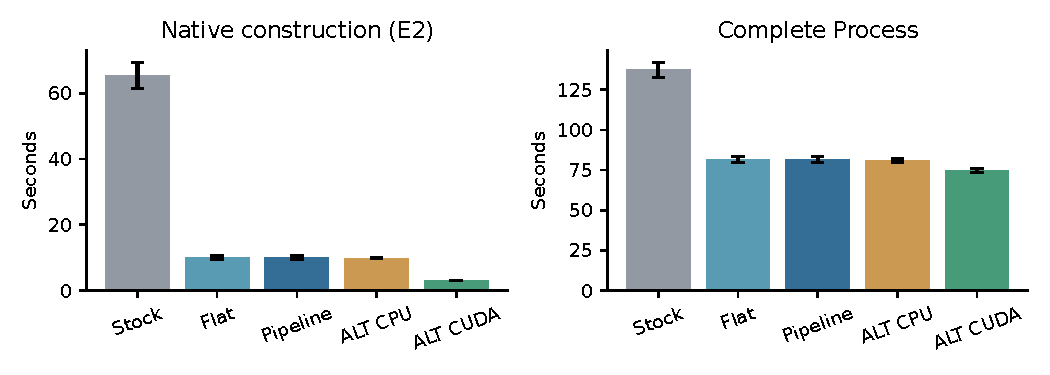
\includegraphics[width=.96\textwidth]{figures/native.pdf}
\caption{LSTM native construction and complete Process (same cohort as Table~\ref{tab:lstm}). Bars show means, error bars sample SD. E2 and Process are nested scopes and are not added.}\label{fig:native}\end{figure*}

The main GPU comparison is against Pipeline: \LstmPipeBuild\ E2 and \LstmPipeProc\ Process acceleration. Against Flat, the corresponding ratios are \LstmFlatBuild\ and \LstmFlatProc. Against the same original ALT algorithm on CPU, CUDA obtains \LstmAltCpuBuild\ and \LstmAltCpuProc. The last Process SD is retained beyond three decimal places because rounding it to zero would hide observed variability. ALT CPU is close to Pipeline here; its different search contract alone does not explain the GPU speedup.

Stock/CUDA gives \LstmStockBuild\ and \LstmStockProc, but these large ratios include the entire implementation combination and cannot be attributed entirely to the CUDA kernel. The smaller Process gain against Pipeline is the relevant system result: loading, initialization, routing and checking remain after accelerating lookahead. Absolute values in Table~\ref{tab:lstm} expose that difference instead of promoting an isolated kernel ratio as full-flow acceleration.

\subsection{Semantics, QoR and Size-Dependent Results}
\begin{table}[t]\centering\caption{LSTM qualification objects. All three map-word difference counts are against Flat.}\label{tab:qor}
\begin{tabular}{lr}\toprule Object / metric & Observation\\\midrule
\tableinput{tables/qor.tex}
\bottomrule\end{tabular}\end{table}

Table~\ref{tab:qor} separates agreement objects. ALT CPU and CUDA agree on complete samples and final wire maps, but their route SHAs differ. Each route independently retains identity during readback. Against Flat, ALT changes 23,111 congestion words with no delay or missing-state changes. A strict-delay native tie rule and ALT's whole-pair lexicographic improvement are different contracts; good measured CPD/WL does not erase that difference. Equal delay words also do not establish equality of all intermediate labels or traversal histories.

\begin{table}[t]\centering\caption{R6.1 Flat/ALT CUDA paired speedup, mean $\pm$ sample SD ($n=3$). This older worker is separate from LSTM and R6.2 Pipeline supplements.}\label{tab:legacy}
\begin{tabular}{lrr}\toprule Case & E2 speedup & Process speedup\\\midrule
\tableinput{tables/legacy.tex}
\bottomrule\end{tabular}\end{table}

BNN supports a second large native result, but only against its measured Flat control (Table~\ref{tab:legacy}). R6.2's old-case Pipeline supplements pass map/QoR checks on another worker and do not complete a missing same-block Pipeline/CUDA comparison for BNN. Even P1 Pipeline and P2 original CUDA on the new worker cannot be paired by matching repeat numbers: they are separate stages.

The s38417 result is deliberately retained: CUDA is slower for both E2 and Process than Flat. A fixed device initialization cost, scans and launches can overwhelm a small build. Original ALT CPU is useful for its construction, while Stock remains fastest for its full Process in that cohort. These observations motivate explicit CPU/GPU choice and size-aware future selection, not a claimed automatic selector or an oracle choosing the fastest measured arm after execution. Three repeats of LSTM plus two legacy cases do not establish all-size or cross-architecture generality.

\subsection{Conversion Dominates Remaining Search Opportunity}
BNN R6.1 repeat 1 has E2=3.104359912 s, E1=0.363794840 s and Process=67.304850295 s. Keeping everything else fixed, eliminating E1 yields at most $E2/(E2-E1)=1.132744\times$ construction or $Process/(Process-E1)=\StageProcBound\times$ Process acceleration. These are conditional bounds for that one process; they do not prohibit redesigning conversion or preparation.

The sole non-formal BNN profile measures E2=3.142660 s, conversion=1.435082 s, prepare=0.787266 s and E1=0.365164 s. Dense mapping/job/cost construction occupies 0.811780 s inside conversion, and H2D occupies 0.118766 s inside prepare. These parent/child intervals must not be stacked together. Preparation includes more than PCIe. No stage medians from different processes are assembled into a synthetic run.

One profile-selected candidate pre-indexes IPIN IDs and fills the same original dense qid-by-node array. It changes construction traversal, not representation. Four affected CPU/CUDA qualifications preserve complete input/output bytes on BNN and s38417. Three CUDA pairs give BNN E2 $1.082\pm0.037\times$, but Process $1.009\pm0.019\times$ has mixed direction; small-case E2/Process also lack consistent gains. Defaults remain unchanged. This secondary ablation is neither qualified on LSTM nor multiplied into its speedup.

\section{Limitations and Hardware Boundary}
The STRICT proposition covers wire-map semantics under explicit assumptions. ALT provides measured CPU/CUDA agreement and qualified downstream behavior on the tested inputs, with congestion counterexamples to native equivalence. Wider seed, architecture and numerical-domain claims would require new evidence. LSTM is an ALT-tuning holdout from the same architecture family and previously appeared in the CPU study. Shared instances, small repetition counts and uncontrolled filesystem caches limit interpretation of variability and deployment performance.

No FPGA hardware superiority is verified. The current candidate lacks an achieved implementation frequency and calibrated dependent random whole-pair RMW service. U280 logical storage totals and software cache hit counts do not establish ports, arbitration, finite queues, cross-SLR placement or service throughput. The observed environment has no visible FPGA or usable installed platform. The hardware state remains \texttt{UNRESOLVED}: specifically, no supported memory-service evidence. Both board-measured acceleration and FPGA-superiority flags remain false.

A separate offline compact-CUDA E1 target and modeled proposal traffic imply necessary service bounds, not native hardware performance; compact/direct native qualification is not inherited. Restarting hardware work would require an actual target/shell or calibrated facility, dependent random 32-byte RMW with finite outstanding requests, a complete physical/timing budget, and end-to-end margin against the strongest matched software baseline. This paper's measured contribution is CPU/GPU lookahead construction, not successful FPGA acceleration or a proof that every FPGA mapping must fail.

\section{Conclusion}
Layer-aware lookahead exposes useful parallelism at two levels, with different semantic obligations. STRICT preserves native sample behavior while removing group barriers through private floods and ordered reduction. ALT exposes search-internal parallelism through a separate whole-pair FP32 wave contract. Native experiments connect sample/map checks, legal routes and QoR to complete construction and Process measurements. The LSTM same-family tuning holdout demonstrates improvement over optimized Pipeline, while BNN and s38417 delimit the observed size-dependent benefit. Construction gains are larger than Process gains, and hardware superiority remains an open, evidence-gated goal.
\clearpage
\bibliographystyle{IEEEtran}
\bibliography{references}
\end{document}
